\documentclass[11pt]{opticajnl}
\journal{opticajournal} 

\setboolean{shortarticle}{true}


\usepackage{lineno}
\usepackage{multicol}

%\linenumbers % Turn off line numbering for Optica Open preprint submissions.

\title{El Guachinche}

%\author[1,2,3]{Luis Ardévol Mesa, Carlos Martínez García \\ \copyrightstatement}
\author[1,2,3]{Luis Ardévol Mesa, Carlos Martínez García, Miguel Mato Martínez}

\begin{document}

\maketitle

\tableofcontents

\hrulefill

\section{Introducción}

Los \textit{guachinches} son establecimientos (en la propia vivienda del propietario) que surgen en la zona del norte del Tenerife como solución para vender el excedente de vino de cada cosecha. El vino se acompaña típicamente con platos tradicionales de la cocina canaria. Actualmente, según el Decreto 83/2013\footnote{\url{https://www.gobiernodecanarias.org/boc/2013/153/001.html}}, hay una regulación muy estricta amparando a estos locales y al viticultor; muchos establecimientos comúnmente denominados ``guachinches'', entran dentro de la categoría \textit{restaurante}, al salirse de lo establecido en este decreto. \\

El Guachinche nace de una idea sencilla pero atractiva: traer el espíritu de los tradicionales guachinches canarios al resto de España, pero con un toque especial. En nuestra cocina, las recetas isleñas comparten protagonismo con una cuidada selección de arepas para todos los públicos, todo esto acompañado de los mejores vinos de las Islas. Es ese equilibrio entre tradición y adaptación lo que nos hace únicos: cada local incorpora platos de la región, porque creemos que la gastronomía local es parte fundamental de nuestra historia. \\

No obstante, quien entra a El Guachinche no solo viene a comer. Para dar una experiencia lo más cercana posible y crear una atmósfera atractiva y familiar para los comensales, nuestros locales presentan una ambientación tradicional y hogareña. La experiencia no sería completa de no ser por nuestro personal, siempre cercano. \\

Actualmente, El Guanchinche cuenta con 13 locales, repartidos en Canarias (7), Galicia (2), Andalucía (2) y Comunidad Valenciana (2). El crecimiento en los últimos dos años ha sido exponencial, por lo que desde la dirección de la empresa nos vemos en la necesidad de implementar un modelo de inteligenia de negocio que nos permita tomar decisiones basadas en datos, priorizando siempre al cliente. \\

\noindent Los objetivos principales perseguidos por la cadena son los siguientes: 
\begin{itemize}
\item Fidelización de clientes. En esta línea, sería conveniente que la economía de cada local no dependiera de la nueva clientela, ya que la fuente de ingresos sería menos estable. 
\item Mejorar la experiencia general del cliente en nuestros locales. 
\item Adaptar la oferta gastronómica a las preferencias de cada región.
\item Ampliar beneficios, especialmente en las regiones menos rentables actualmente.
\item Estudio de la rentabilidad del servicio a domicilio.
\end{itemize}

El servicio a domicilio corre a cargo de dos empresas: Uber Eats y Glovo. Conocida la comisión de estos servicios, cada local descuenta esta comisión del total y almacena el beneficio real de cada pedido a domicilio. Para cumplir con los objetivos, es importante conocer: 
\begin{itemize}
\item La cantidad de nuevos clientes en comparación a los habituales. 
\item La satisfacción de los clientes con los servicios prestados en nuestros establecimientos.
\item El rendimiento económico de cada uno de los locales, así como de la totalidad de la cadena. Esto incluye:
\begin{itemize}
\item Ventas de cada producto ofertado.
\item Gastos e ingresos de cada local. En estos últimos sería necesario distinguir entre ingresos presenciales e ingresos a domicilio. 
\end{itemize}
\end{itemize}

A continuación, se describen los procesos de diseño y construcción del almacén de datos para gestionar la información necesaria. Posteriormente se comentarán los procesos de extracción, transformación y carga que permiten la creación y actualización del almacén de datos. Se sigue con algunas consultas de interés para los objetivos descritos anteriormente y, para terminar, se incluyen cuadros de mando e informes adecuados al caso de estudio.

\section{Diseño y construcción del almacén de datos}

Nuestros locales llevan un registro cuidadoso de los aspectos más importantes de la actividad diaria, como son las ventas, los gastos o la opinion de los clientes. Cada local genera reportes mensuales que recogen estos datos y son enviados a la central para su análisis. Estos reportes son los que nos permitirán obtener la información necesaria para la toma de decisiones. 

\subsection{Diseño del almacén de datos}

Para realizar el diseño del almacén de datos, es necesario conocer primero la estructura de los datos recogidos en los reportes de cada local. Concretamente, cada mes se reciben dos archivos de datos por cada local de nuestra cadena. El primero de ellos contiene toda la información relacionada con la economía del restaurante: desglose de gastos en cuatro categorías (personal, suministros, alquiler y otros), ingresos por ventas (diferenciando entre los servicios presencial y domicilio) y clientela. Esto será beneficio para varios de los objetivos de la cadena. Siendo un poco más específicos, se proporcionan los siguientes datos:
\begin{itemize}
\item Un identificador entero para cada local, generado por la central en orden de apertura.
\item La fecha de envío del reporte (establecida para el primer día del mes). 
\item Los gastos en alquiler, personal, suministros (proveedores), y extras (limpieza, mantenimiento, etc.), todo en euros.
\item Los ingresos, tanto por vía presencial como a domicilio, en euros. Como ya se ha mencionado, estos ingresos ya tienen descontada la comisión de Uber Eats o Glovo.
\item Los clientes totales por ambos canales, así como el número de clientes nuevos.
\item Los platos ofertados en el local, cada uno con los siguientes datos:
\begin{itemize}
\item Un identificador entero para cada plato, generado por la central.
\item El nombre, precio y número de ventas del plato. 
\end{itemize}
\end{itemize}

Estos datos se recogen en un archivo XML como el que se muestra en la figura \ref{fig:xml_economico}.

\begin{figure}[h]
\centering
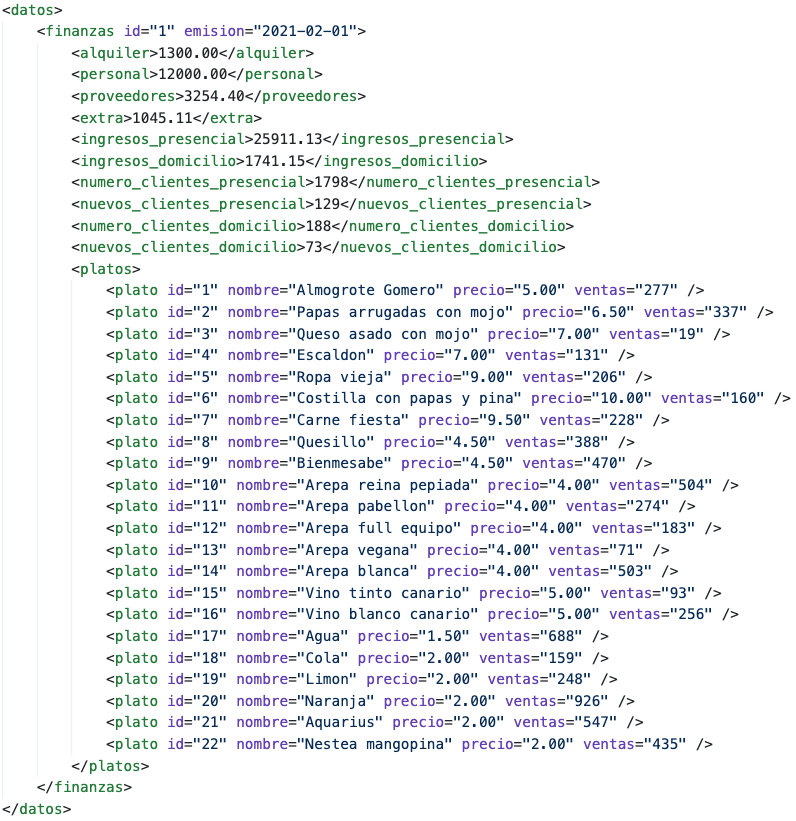
\includegraphics[width=0.6\textwidth]{fotos/1.png}
\caption{Ejemplo de archivo XML con los datos económicos mensuales de un local.}
\label{fig:xml_economico}
\end{figure}

\noindent Los identificadores de los locales son los siguientes:
\begin{multicols}{2}
\begin{itemize}
\item 1: La Laguna, Tenerife.
\item 2: Hermigua, La Gomera.
\item 3: Cotillo, Fuerteventura.
\item 4: Las Palmas de Gran Canaria, Gran Canaria.
\item 5: Tazacorte, La Palma.
\item 6: Valverde, El Hierro.
\item 7: Arrecife, Lanzarote.
\item 8: Granada, Granada.
\item 9: Sevilla, Sevilla.
\item 10: Santiago de Compostela, A Coruña.
\item 11: Vigo, Pontevedra.
\item 12: Alicante, Comunidad Valenciana.
\item 13: Valencia, Comunidad Valenciana. 
\end{itemize}
\end{multicols}

\noindent Los identificadores de los productos son los siguientes:
\begin{multicols}{3}
\begin{itemize}
\item 1: Almogrote Gomero.
\item 2: Papas arrugadas con mojo.
\item 3: Queso asado con mojo.
\item 4: Escaldón.
\item 5: Ropa vieja.
\item 6: Costilla con papas y piña.
\item 7: Carne fiesta.
\item 8: Quesillo.
\item 9: Bienmesabe.
\item 10: Arepa reina pepiada.
\item 11: Arepa pabellón.
\item 12: Arepa full equipo.
\item 13: Arepa vegana.
\item 14: Arepa blanca.
\item 15: Vino tinto canario.
\item 16: Vino blanco canario.
\item 17: Agua.
\item 18: Refresco de cola.
\item 19: Refresco de limón.
\item 20: Refresco de naranja.
\item 21: Aquarius.
\item 22: Nestea mango-piña.
\item 23: Salmorejo.
\item 24: Pescaito frito.
\item 25: Gambitas de Huelva.
\item 26: Pestiños.
\item 27: Vino tinto andaluz.
\item 28: Vino blanco andaluz.
\item 29: Pulpo a feira.
\item 30: Empanada (porción).
\item 31: Lacon con grelos.
\item 32: Tarta de Santiago.
\item 33: Vino tinto gallego.
\item 34: Vino blanco gallego.
\item 35: Paella.
\item 36: Arroz negro.
\item 37: Esgarraet. 
\item 38: Fartons. 
\item 39: Vino tinto valenciano.
\item 40: Vino blanco valenciano.
\end{itemize}
\end{multicols}

Como bien describe el objetivo del negocio, cada región tiene sus platos típicos. Los 22 primeros productos son comunes a todos los locales de la cadena, mientras que a partir de ahí, cada región incorpora distintos productos, como es el caso del \textit{salmorejo} en Andalucía, el \textit{lacçon con grelos} en Galicia o el \textit{esgarraet} en la Comunidad Valenciana. Así mismo, cada local ofrece vinos de proximidad. \\

Para cumplir los objetivos relacionados con la satisfacción y fidelización de clientes, cada local proporciona un segundo archivo, en este caso en formato CSV, con valoraciones de los clientes: en caso de ser clientes presenciales, se valora el ambiente del local, el personal y la calidad de la comida, mientras que los clientes a domicilio simplemente hacen llegar una valoración del servicio general. Así, cada fila del archivo da el identificador del local, la fecha de la valoración, y las votaciones correspondientes (3 en el caso de clientes presenciales, una en el caso de clientes a domicilio). Un ejemplo de este archivo se muestra en la figura \ref{fig:csv_valoraciones}.

\begin{figure}[h]
\centering
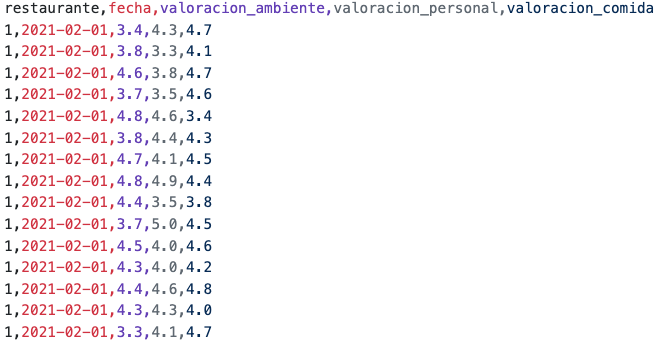
\includegraphics[width=0.6\textwidth]{fotos/2.png}
\caption{Ejemplo de archivo CSV con las valoraciones de los clientes de un local.}
\label{fig:csv_valoraciones}
\end{figure}

Se dará a los datos almacenados de cada uno de los archivos anteriores la máxima granularidad posible, es decir, mensual. Las dimensiones seleccionadas son las siguientes:
\begin{itemize}
\item \textbf{Tiempo}: la dimensión temporal de los datos se representa mediante dos niveles: año y mes.
\item \textbf{Restaurante}: la dimensión restaurante actúa como dimensión geográfica. Se tendrán en cuenta todos los locales de la cadena y se mostrarán dos niveles, uno para el país y otro para la ciudad.
\item \textbf{Producto}: la dimensión producto recoge todos los platos ofertados en los locales de la cadena. Esta es una dimensión plana que muestra los productos y el precio asociado a cada uno de ellos.
\end{itemize}
\noindent Los hechos seleccionados para el almacén de datos son los siguientes:
\begin{itemize}
\item \textbf{Finanzas}: se almacenan los costes e ingresos de los locales, junto con los datos de los clientes para cada combinación de las siguientes dimensiones: tiempo (mes de envío de los reportes) y restaurante (mediante el identificador de cada local).
\item \textbf{Producto}: se almacenan los hechos relacionados con las ventas de los productos ofertados en los locales, para cada combinación de las siguientes dimensiones: tiempo (mes de envío de los reportes), restaurante (mediante el identificador de cada local) y producto (mediante el identificador de cada plato). Se tiene el númer ototal de ventas mensuales de un producto, así como un cálculo de los ingresos generados por ese producto, a partir de sus ventas y su precio.
\item \textbf{Feedback}: se almacenan las valoraciones de los clientes para cada combinación de las siguientes dimensiones: tiempo (mes de envío de los reportes) y restaurante (mediante el identificador de cada local). Se almacena la media de las valoraciones de los clientes para cada uno de los aspectos recogidos en los reportes.
\end{itemize}

Por tanto, el modelo conceptual del almacén de datos se muestra en la figura \ref{fig:esquema_almacen}, siendo un esquema con tres estrellas y tres dimensiones.

\begin{figure}[h]
\centering
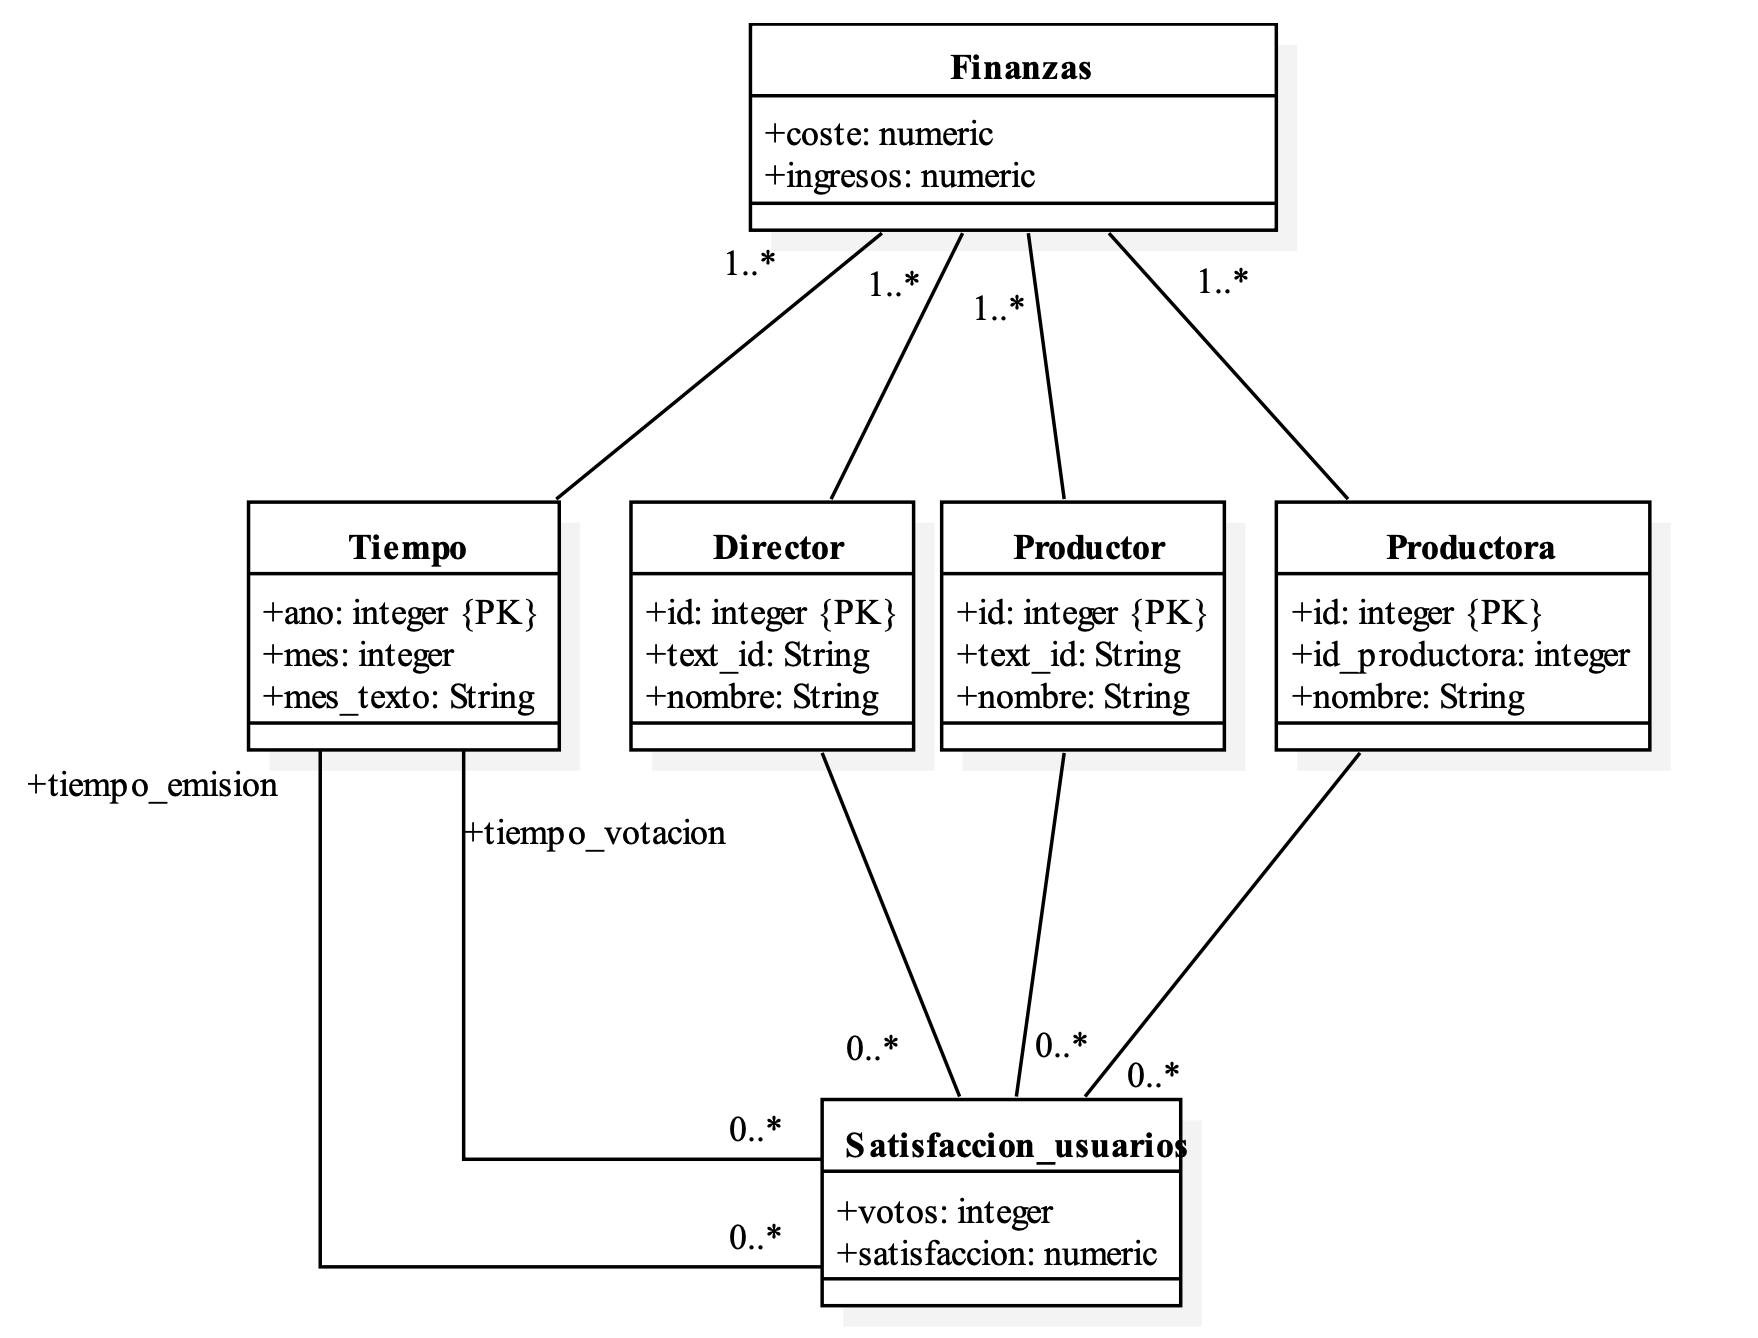
\includegraphics[width=0.7\textwidth]{fotos/3.png}
\caption{Esquema conceptual del almacén de datos. \textcolor{red}{Hacer el bueno}}
\label{fig:esquema_almacen}
\end{figure}

Los detalles de la implementación del almacén de datos se describen en la siguiente tabla: 

\begin{table}[H]
\centering
\begin{tabular}{cll}
\hline
\multicolumn{3}{|c|}{Dimensiones} \\ \hline
\multicolumn{1}{l}{} & & \\ \hline
\multicolumn{3}{|c|}{Tiempo} \\ \hline \hline
\multicolumn{1}{|c}{Atributo} & \multicolumn{1}{c}{Tipo} & \multicolumn{1}{c|}{Descripción} \\ \hline
\multicolumn{1}{|l}{id (pk)} & Integer & \multicolumn{1}{l|}{\begin{tabular}[c]{@{}l@{}}Identificador autoincremental generado por el almacén \\ cada vez que se inserta un nuevo mes. \end{tabular}} \\ 
\multicolumn{1}{|l}{} &  & \multicolumn{1}{l|}{\begin{tabular}[c]{@{}l@{}}\end{tabular}} \\ \hline
\multicolumn{1}{|l}{ano} & Integer & \multicolumn{1}{l|}{\begin{tabular}[c]{@{}l@{}}Número correspondiente al año. \end{tabular}} \\ \hline
\multicolumn{1}{|l}{mes} & Integer & \multicolumn{1}{l|}{\begin{tabular}[c]{@{}l@{}}Número correspondiente al mes dentro del año. \end{tabular}} \\ \hline
\multicolumn{1}{|l}{mes\_texto} & String & \multicolumn{1}{l|}{\begin{tabular}[c]{@{}l@{}}Texto con el nombre del mes. \end{tabular}} \\ \hline
\multicolumn{1}{l}{} &  & \\ \hline
\multicolumn{3}{|c|}{Restaurante} \\ \hline \hline
\multicolumn{1}{|c}{Atributo} & \multicolumn{1}{c}{Tipo} & \multicolumn{1}{c|}{Descripción} \\ \hline
\multicolumn{1}{|l}{id (pk)} & Integer & \multicolumn{1}{l|}{\begin{tabular}[c]{@{}l@{}}Identificador de cada local, generado por la central. \end{tabular}} \\ 
\multicolumn{1}{|l}{} &  & \multicolumn{1}{l|}{\begin{tabular}[c]{@{}l@{}}\end{tabular}} \\ \hline
\multicolumn{1}{|l}{pais} & String & \multicolumn{1}{l|}{\begin{tabular}[c]{@{}l@{}}País donde se sitúa el local. \end{tabular}} \\ \hline
\multicolumn{1}{|l}{ciudad} & String & \multicolumn{1}{l|}{\begin{tabular}[c]{@{}l@{}}Ciudad donde se sitúa el local. \end{tabular}} \\ \hline
\multicolumn{1}{l}{} &  & \\ \hline
\multicolumn{3}{|c|}{Producto} \\ \hline \hline
\multicolumn{1}{|c}{Atributo} & \multicolumn{1}{c}{Tipo} & \multicolumn{1}{c|}{Descripción} \\ \hline
\multicolumn{1}{|l}{id (pk)} & Integer & \multicolumn{1}{l|}{\begin{tabular}[c]{@{}l@{}}Identificador de cada plato, generado por la central. \end{tabular}} \\ \hline 
\multicolumn{1}{|l}{nombre} & String & \multicolumn{1}{l|}{\begin{tabular}[c]{@{}l@{}}Nombre del plato. \end{tabular}} \\ \hline
\multicolumn{1}{|l}{precio} & Numeric & \multicolumn{1}{l|}{\begin{tabular}[c]{@{}l@{}}Precio del plato. \end{tabular}} \\ \hline
\multicolumn{1}{l}{} &  & \\
\multicolumn{1}{l}{} &  & \\
\end{tabular}
\end{table}

\begin{table}[H]
\centering
\begin{tabular}{cll}
\hline
\multicolumn{3}{|c|}{Hechos} \\ \hline
\multicolumn{1}{l}{} & & \\ \hline
\multicolumn{3}{|c|}{Finanzas} \\ \hline \hline
\multicolumn{1}{|c}{Atributo} & \multicolumn{1}{c}{Tipo} & \multicolumn{1}{c|}{Descripción} \\ \hline
\multicolumn{1}{|l}{alquiler} & Numeric & \multicolumn{1}{l|}{\begin{tabular}[c]{@{}l@{}}Gasto en alquiler de un local, en euros. \end{tabular}} \\ \hline
\multicolumn{1}{|l}{personal} & Numeric & \multicolumn{1}{l|}{\begin{tabular}[c]{@{}l@{}}Gasto en personal de un local, en euros. \end{tabular}} \\ \hline
\multicolumn{1}{|l}{proveedores} & Numeric & \multicolumn{1}{l|}{\begin{tabular}[c]{@{}l@{}}Gasto en suministros de un local, en euros. \end{tabular}} \\ \hline
\multicolumn{1}{|l}{extra} & Numeric & \multicolumn{1}{l|}{\begin{tabular}[c]{@{}l@{}}Gasto en extras de un local, en euros. \end{tabular}} \\ \hline
\multicolumn{1}{|l}{ingresos\_presencial} & Numeric & \multicolumn{1}{l|}{\begin{tabular}[c]{@{}l@{}}Ingresos por ventas presenciales de un local, en euros. \end{tabular}} \\ \hline
\multicolumn{1}{|l}{ingresos\_domicilio} & Numeric & \multicolumn{1}{l|}{\begin{tabular}[c]{@{}l@{}}Ingresos por ventas a domicilio de un local, en euros. \end{tabular}} \\ \hline
\multicolumn{1}{|l}{numero\_clientes\_presencial} & Integer & \multicolumn{1}{l|}{\begin{tabular}[c]{@{}l@{}}Número total de clientes presenciales de un local. \end{tabular}} \\ \hline
\multicolumn{1}{|l}{numero\_clientes\_domicilio} & Integer & \multicolumn{1}{l|}{\begin{tabular}[c]{@{}l@{}}Número total de clientes a domicilio de un local. \end{tabular}} \\ \hline
\multicolumn{1}{|l}{nuevos\_clientes\_presencial} & Integer & \multicolumn{1}{l|}{\begin{tabular}[c]{@{}l@{}}Número de clientes presenciales nuevos de un local. \end{tabular}} \\ \hline
\multicolumn{1}{|l}{nuevos\_clientes\_domicilio} & Integer & \multicolumn{1}{l|}{\begin{tabular}[c]{@{}l@{}}Número de clientes nuevos a domicilio de un local. \end{tabular}} \\ \hline
\multicolumn{1}{l}{} &  & \\ \hline
\multicolumn{3}{|c|}{Producto} \\ \hline \hline
\multicolumn{1}{|c}{Atributo} & \multicolumn{1}{c}{Tipo} & \multicolumn{1}{c|}{Descripción} \\ \hline
\multicolumn{1}{|l}{ventas} & Integer & \multicolumn{1}{l|}{\begin{tabular}[c]{@{}l@{}}Número total de ventas de un producto en un local. \end{tabular}} \\ \hline
\multicolumn{1}{l}{} &  & \\ \hline
\multicolumn{3}{|c|}{Feedback} \\ \hline \hline
\multicolumn{1}{|c}{Atributo} & \multicolumn{1}{c}{Tipo} & \multicolumn{1}{c|}{Descripción} \\ \hline
\multicolumn{1}{|l}{valoracion\_ambiente} & Numeric & \multicolumn{1}{l|}{\begin{tabular}[c]{@{}l@{}}Valoración promedio (entre 0 y 5 con un decimal) \\ del ambiente de un local, según sus clientes. \end{tabular}} \\ \hline
\multicolumn{1}{|l}{valoracion\_personal} & Numeric & \multicolumn{1}{l|}{\begin{tabular}[c]{@{}l@{}}Valoración promedio (entre 0 y 5 con un decimal) \\ del personal de un local, según sus clientes. \end{tabular}} \\ \hline
\multicolumn{1}{|l}{valoracion\_comida} & Numeric & \multicolumn{1}{l|}{\begin{tabular}[c]{@{}l@{}}Valoración promedio (entre 0 y 5 con un decimal) \\ de la calidad de la comida de un local, según sus clientes. \end{tabular}} \\ \hline
\end{tabular}
\caption{Borrar esto: Básicamente en cada tabla de estas habrá una fila por cada restaurante y por cada mes y año.}
\end{table}

\newpage 

\subsection{Creación de los cubos de datos}

Utilizando como base las estructuras de datos relacionales descritas en el apartado anterior, se crea un esquema multidimensional con tres cubos y tres dimensiones compartidas entre ellos. Estas se definen a nivel de esquema y posteriormente se reutilizan a nivel de cubo:

\begin{itemize}
\item Dimensión: \textbf{Tiempo}. Dimensión de tipo temporal.
\begin{itemize}
\item Jerarquía: \textit{jerarquiaTiempo}. Definida por el atributo \textit{id}. 
\begin{itemize}
\item Nivel: \textit{ano}. Nivel de tipo \textit{TimeYears} definido por el atributo \textit{ano}.
\item Nivel: \textit{mes}. Nivel de tipo \textit{TimeMonths} definido por el atributo \textit{mes}. Se utiliza el atributo \textit{mes\_texto} para nombrar a los elementos de este nivel.
\item Tabla: tiempo
\end{itemize}
\end{itemize}
\item Dimensión: \textbf{Restaurante}. Dimensión de tipo estándar.
\begin{itemize}
\item Jerarquía: \textit{jerarquiaRestaurantes}. Definida por el atributo \textit{id}.
\begin{itemize}
\item Nivel: \textit{pais}. Nivel de tipo regular definido por el atributo \textit{pais}.
\item Nivel: \textit{ciudad}. Nivel de tipo regular definido por el atributo \textit{ciudad}.
\item Tabla: restaurante
\end{itemize}
\end{itemize}
\item Dimensión: \textbf{Producto}. Dimensión de tipo estándar.
\begin{itemize}
\item Jerarquía: \textit{jerarquiaProductos}. Definida por el atributo \textit{id}.
\begin{itemize}
\item Nivel: \textit{nombre}. Nivel de tipo regular definido por el atributo \textit{nombre}.
\item Tabla: producto
\end{itemize}
\end{itemize}
\item Cubo: \textbf{Finanzas}. 
\begin{itemize}
\item Tabla: \textit{finanzas}
\item Dimensiones 
\begin{itemize}
\item Dimensión usada: \textbf{Tiempo}. Se referencia a la dimensión \textit{Tiempo}. Se utiliza el atributo \textit{fecha} como clave foránea.
\item Dimensión usada: \textbf{Restaurante}. Se referencia a la dimensión \textit{Restaurante}. Se utiliza el atributo \textit{restaurante} como clave foránea.
\end{itemize}
\item Medidas \textcolor{red}{MIRAR BIEN PORQUE NO SE AGREGAN ?}
\begin{itemize}
\item Medida: \textbf{Alquiler}. ??
\item Medida: \textbf{Personal}. ??
\item Medida: \textbf{Proveedores}. ??
\item Medida: \textbf{Extra}. ??
\item Medida: \textbf{Ingresos presencial}. ??
\item Medida: \textbf{Ingresos domicilio}. ??
\item Medida: \textbf{Número clientes presencial}. ??
\item Medida: \textbf{Número clientes domicilio}. ??
\item Medida: \textbf{Nuevos clientes presencial}. ??
\item Medida: \textbf{Nuevos clientes domicilio}. ??
\item Medida calculada: \textbf{Gastos totales}. Se genera un nuevo valor para la dimensión \textit{Measures} usando la expresión MDX: ``[Measures].[Alquiler] + [Measures].[Personal] + [Measures].[Proveedores] + [Measures].[Extra]''
\item Medida calculada: \textbf{Ingresos totales}. Se genera un nuevo valor para la dimensión \textit{Measures} usando la expresión MDX: ``[Measures].[Ingresos presencial] + [Measures].[Ingresos domicilio]''
\item Medida calculada: \textbf{Beneficio}. Se genera un nuevo valor para la dimensión \textit{Measures} usando la expresión MDX: ``[Measures].[Ingresos totales] - [Measures].[Gastos totales]''
\item Medida calculada: \textbf{Número total clientes}. Se genera un nuevo valor para la dimensión \textit{Measures} usando la expresión MDX: ``[Measures].[Número clientes presencial] + [Measures].[Número clientes domicilio]''
\item Medida calculada: \textbf{Número total nuevos clientes}. Se genera un nuevo valor para la dimensión \textit{Measures} usando la expresión MDX: ``[Measures].[Nuevos clientes] + [Measures].[Nuevos clientes domicilio]''
\item Medida calculada: \textbf{Beneficio por cliente}. Se genera un nuevo valor para la dimensión \textit{Measures} usando la expresión MDX: ``[Measures].[Beneficio] / [Measures].[Número total clientes]''
\end{itemize}
\end{itemize}
\item Cubo: \textbf{Producto}.
\begin{itemize}
\item Tabla: \textit{producto}
\item Dimensiones
\begin{itemize}
\item Dimensión usada: \textbf{Tiempo}. Se referencia a la dimensión \textit{Tiempo}. Se utiliza el atributo \textit{fecha} como clave foránea.
\item Dimensión usada: \textbf{Restaurante}. Se referencia a la dimensión \textit{Restaurante}. Se utiliza el atributo \textit{restaurante} como clave foránea.
\item Dimensión usada: \textbf{Producto}. Se referencia a la dimensión \textit{Producto}. Se utiliza el atributo \textit{producto} como clave foránea.
\end{itemize}
\item Medidas \textcolor{red}{como trato a precio? lo meto en la dimension producto?}
\begin{itemize}
\item Medida: \textbf{Ventas}. ??
\item Medida calculada: \textbf{Ingresos por producto}. Se genera un nuevo valor para la dimensión \textit{Measures} usando la expresión MDX: ``[Measures].[Ventas] * [Producto].[precio]''
\end{itemize}
\end{itemize}
\item Cubo: \textbf{Feedback}.
\begin{itemize}
\item Tabla: \textit{feedback}
\item Dimensiones
\begin{itemize}
\item Dimensión usada: \textbf{Tiempo}. Se referencia a la dimensión \textit{Tiempo}. Se utiliza el atributo \textit{fecha} como clave foránea.
\item Dimensión usada: \textbf{Restaurante}. Se referencia a la dimensión \textit{Restaurante}. Se utiliza el atributo \textit{restaurante} como clave foránea.
\end{itemize}
\item Medidas
\begin{itemize}
\item Medida: \textbf{Valoración ambiente}. Se agrega el atributo \textit{valoracion\_ambiente} usando la funcion AVG.
\item Medida: \textbf{Valoración personal}. Se agrega el atributo \textit{valoracion\_personal} usando la funcion AVG.
\item Medida: \textbf{Valoración comida}. Se agrega el atributo \textit{valoracion\_comida} usando la funcion AVG.
\item Medida calculada: \textbf{Valoración media restaurante}. Se genera un nuevo valor para la dimensión \textit{Measures} usando la expresión MDX: ``([Measures].[Valoración ambiente] + [Measures].[Valoración personal] + [Measures].[Valoración comida]) / 3''
\end{itemize}
\end{itemize}
\end{itemize}

\section{Extracción, transformación y carga de datos}

\section{Análisis de datos con MDX y ROLAP}

\subsection{Consultas MDX}

\subsection{Consultas ROLAP}

\section{Cuadros de mando e informes}

\end{document}

